\documentclass[10pt,twocolumn]{article}
\usepackage[utf8]{inputenc}
\usepackage{graphicx}
\usepackage{amsmath}
\usepackage{amssymb}
\usepackage{hyperref}
\usepackage{geometry}
\usepackage[table]{xcolor}
\usepackage{cite}

\definecolor{verylightgray}{gray}{0.85}

\geometry{margin=1in}

\title{Improving Model Inversion Using Additional Backbones}
\author{Christopher Roßbach \\ FAU-Erlangen-Nürnberg}
\date{\today}

\begin{document}

\maketitle
\begin{abstract}
    Model inversion, or feature inversion, seeks to reconstruct the original input of a neural network from its outputs or intermediate representations.
    This process is highly ill-posed, especially when reconstructing images from deep feature embeddings, and thus requires strong priors and constraints to yield plausible results.
    In this work, we investigate optimization-based methods for reconstructing images from their embeddings in various vision model latent spaces.
    Building on empirical observations, we propose a novel approach that leverages the embeddings of multiple reconstruction candidates across different backbone models to improve reconstruction quality.
    Our results motivate further work on how incorporating information from foreign backbones can enhance reconstruction fidelity.
\end{abstract}

\section{Introduction}
The reconstruction of network inputs from intermediate representations produced by a model can be used to evaluate the privacy risks of sharing such representations.
Due to the ill-posed nature of the problem, one may expect that the reconstruction of the input is not possible in practice and thus share such representations without caution.
As the private input may contain sensitive or private information, the ability to reconstruct the input from such representations poses a significant privacy risk.
As such, one can consider the reconstruction of the input from intermediate representations as an attack on the privacy of the victim owning the input data.
This report investigates techniques that try to reconstruct the full model input from a latent representation.
We limit ourselves to the task of image reconstruction from feature embeddings given by a pretrained vision backbone.
We assume a white-box setting where the attacker has access to the model architecture and parameters as well as the feature embedding of the target image.

We aim to approximate the private image $x^*$ owned by the victim from its embedding $y^* = f(x^*)$.
We assume that both, the network $f$ and the embedding $y^*$ are known to the attacker (either leaked or purposely shared).

To leverage the information contained in the model $f$, we employ an optimization-based approach that iteratively refines a reconstruction proposal $\hat{x}$ to minimize the distance between its embedding $f(\hat{x})$ and the target $y^*$.
To address the inherent ambiguity of the inversion process, we propose incorporating additional information from foreign backbones $h$ by encouraging the reconstructions to have similar embeddings under $h$.
Empirically, we observe that embeddings of different reconstruction candidates under a foreign backbone tend to scatter around the true embedding $h(x^*)$.
By leveraging this property, we intent to improve reconstruction quality, by pulling the embeddings of the reconstruction candidates closer together.
Our findings show clear trends in different dimensions of the reconstruction process, including the choice of foreign backbone, the method of aggregating embeddings, the number of parallel reconstructions used and the effect of the data distribution.

\section{Methodology}
We try to reconstruct the private image from its embedding through an optimization process.
The problem of reconstructing the private image from its embedding is a strongly ill posed which forces us to incorporate additional constraints and priors to the optimization process.
The optimization problem can be formulated as
$$
\min_{\hat{x}} d_f(f(\hat{x}), y^*) + \mathcal{R}(\hat{x}),
$$
where $\mathcal{R}$ is a regularization term that encourages the reconstruction to be smooth and natural and is further described in Section~\ref{reg}.
$d_f$ is a distance function that is dependent on the used backbone $f$.
For a ResNet backbone we use the mean squared error (MSE) as the distance function while using a cosine based distance for a clip encoder.
\subsection{The Iterative Base Method}\label{base_method}
We employ an iterative optimization method to progressively refine the reconstruction.
We generally optimize in the image space while resorting to a lower dimensional image space at the beginning of the reconstruction.
Successive upscaling encourages the reconstruction of coarse structures before refining details.
We take the resolution steps used in~\cite{kazemiWhatWeLearn2024} and find adding another low resolution step of 32 to be beneficial, resulting in a scale sequence of $n\in\{32, 64, 128, 224\}$ where upscaling is performed at steps 400, 900 and 1800.

At each iteration, we update the reconstruction $x$ in the possibly smaller space $\mathbb{R}^{3\times n \times n}$ from which we retrieve the full size reconstruction proposal $\mathbb{R}^{3\times N \times N}\ni\hat{x} = S_N(x)$ by using a differentiable scaling function $S_k:\mathbb{R}^{3\times n \times n}\rightarrow\mathbb{R}^{3\times k \times k}$.
The next reconstruction $x$ is determined by
\begin{equation}\label{eq:update_rule}
x^{(t)} = S_{n_t}\left(x^{(t-1)} - \eta \dfrac{\nabla \mathcal{L}(x^{(t-1)}, y^*)}{\|\nabla \mathcal{L}(x^{(t-1)}, y^*)\|_2}\right),
\end{equation}
where $t$ denotes the iteration step, $n_t$ the resolution at step $t$, $\eta$ is the learning rate, and $\mathcal{L}$ the loss function.
This process is repeated for 3000 iterations after which no notable improvement was noticed in practice.
Normally we perform multiple reconstructions in parallel, because the result depends on the initialization $x^{(0)}$.
We denote such a set of equally constructed reconstructions as $X^{(t)} = \{x^{(t)}_0, x^{(t)}_1, \dots, x^{(t)}_{m-1}\}$ where $m$ is the number of parallel reconstructions.

For now, the loss function $\mathcal{L}$ is defined as
\begin{equation}\label{eq:loss_function_base}
\mathcal{L}(x, y^*) = \mathcal{L}_{f}(x, y^*) + \mathcal{R}(S_N(x)),
\end{equation}
with
\begin{equation}\label{eq:loss_function_f}
    \mathcal{L}_f(x, y^*) = d_{f}(f(A(S_N(x))), y^*),
\end{equation}
where $A$ is a randomized augmentation function as described in Section~\ref{augs}, and $d_f$ is a distance function that is dependent on the used backbone $f$ and $\mathcal{R}$ is a regularization term as described in Section~\ref{reg}.

\subsection{Augmentations}\label{augs}
As proposed in~\cite{ghiasiPlugInInversionModelAgnostic2021} we employ a set of differentiable augmentations to improve the robustness of the reconstruction.
We expect the embedding to be stable under (slight) scaling, rotation and translation.
We incorporate these augmentations into the optimization process as a prior by applying a (different) set of augmentations at each step of the optimization.
The transformation is thereby chosen randomly from $(\text{scale}, \text{rotate}, \text{translate}_h, \text{translate}_v) \in \lbrack 0.7, 1.5\rbrack\times \lbrack -30, 30\rbrack \times \lbrack -0.1, 0.1\rbrack \times \lbrack -0.1, 0.1\rbrack$.

\subsection{Regularization}\label{reg}
For regularization we use a term based on total variation as proposed in~\cite{mahendranUnderstandingDeepImage2015} with the adjustment of using a $L_1$ distance:
$$
\mathcal{R}(x) = g_{\alpha,\beta}\left(\dfrac{\mathcal{R}_{TV}(x)}{(n-1)^2}\right)
$$
with
$$
\mathcal{R}_{TV}(x) = \sum_{i,j} \left| x_{i,j} - x_{i + 1,j} \right| + \left| x_{i,j} - x_{i,j + 1} \right|.
$$
This term is used to penalize sharp edges in the reconstructed images.
Here $n$ refers to the width of the square image and $g_{\alpha,\beta}$ is a penalty function that balances the contribution of the total variation term and is defined as:
$$
g_{\alpha,\beta}(x) = \text{relu}(x - \alpha) + \beta\cdot\text{relu}(x - \alpha) ^ 2.
$$
This quadratic dead zone penalty function allows for punishment-free variation in the interval $\lbrack-\alpha,\alpha\rbrack$ and (for big enough $\beta$) limits the total variation to be close to $\alpha$.
The use of this penalty function makes sure, that the this regularization term does not loose importance when adding additional terms to the objective function of the optimization.
A parameter selection of $\alpha = 0.3$ and $\beta = 10$ was found to yield good results in practice.

\subsection{Impact of Inverted Model}
The reconstruction method described in Section~\ref{base_method} yields visibly different results when using different backbones $f$.
It is to note, that the reconstruction for different backbones does not strictly yield better or worse reconstructions, but rather reconstruction with qualitatively different details.
This effect can be seen in figure~\ref{fig:resnet_vs_clip}.

For the picture of the safe, we note that the reconstruction on a ResNet backbone gives a picture containg structural properties of a safe, while the reconstruction on the clip embedding seems to reproduce the text contained in the lower right corner of original picture.
For the dog picture, the reconstruction based on the clip embedding yields a better representation of the dog's features compared to the ResNet based reconstruction, while the ResNet reconstruction contains patterns of the background.
In the reconstruction of the fish picture the ResNet based reconstruction focuses on the fish's shape and the hands while the clip based reconstruction reconstructs the face of the person holding the fish.

From this observation we conclude, that a improvement in reconstruction quality can be achieved by combining different backbones in the reconstruction process while maintaining the assumption to have access to a single embedding.
\begin{figure}[ht]
    \centering
    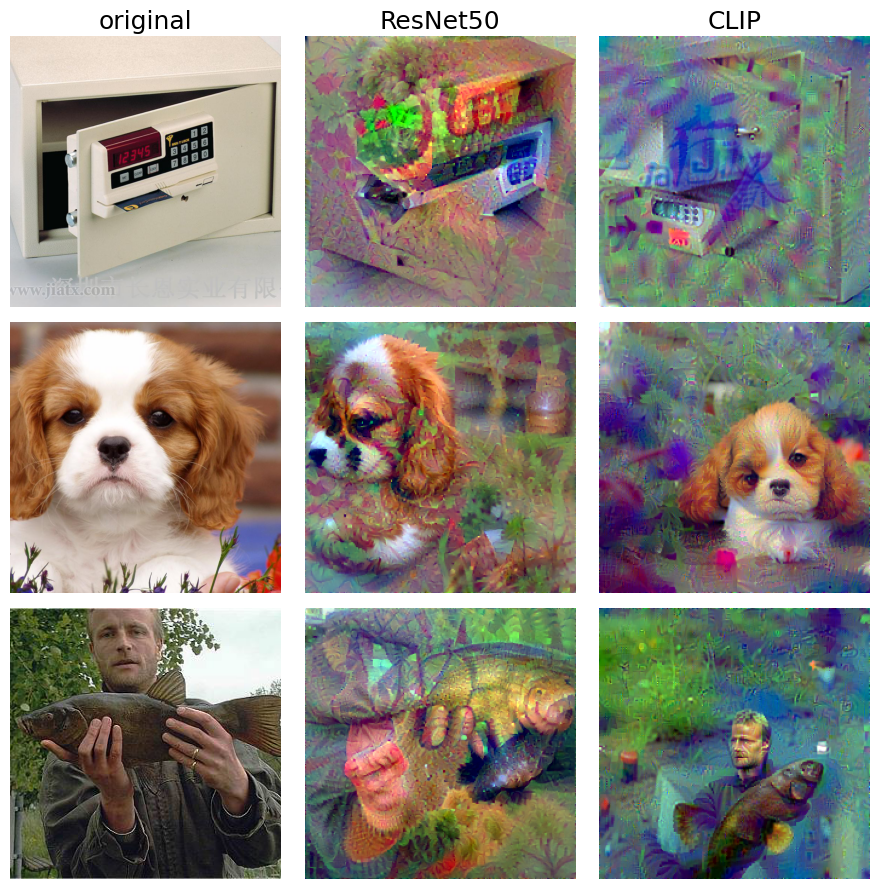
\includegraphics[width=\linewidth]{figures/resnet-vs-clip.png}
    \caption{
        Comparison of reconstructions on ResNet and CLIP backbones.
    }
    \label{fig:resnet_vs_clip}
\end{figure}

\subsection{Average of Foreign Embeddings}
Another important observation is that if we have two different backbones $f$ and $h$, a private image $x^*$ and a slightly modified version $x^*_p$ of the private image for which $f(x^*)\approx f(x^*_p)$ then we also observe $h(x^*)\approx h(x^*_p)$.
That is, if we modify the private image only slightly, the embeddings produced by different backbones remain consistent.
However, this behaviour does not apply to reconstructions: for a reconstruction $\hat x_f$ obtained by procedure described in~\ref{base_method} with respect to the backbone $f$ that suffices $f(\hat x_f)\approx f(x^*)$ we observe strong differences in the embedding under $h$, $d_h(h(\hat x_f),h(x^*)) \gg d_f(f(\hat x_f),f(x^*))\approx 0$.
The same is true for two different reconstructions $\hat x_{f,0}$ and $\hat x_{f,1}$: while $f(\hat x_{f,0})\approx f(\hat x_{f,1})$ we observe $h(\hat x_{f,0})\not\approx h(\hat x_{f,1})$.

Furthermore, if we have a set of reconstruction $X_f = \{\hat x_{f,0}, \hat x_{f,1}, \dots\}$ we observe that that the average embedding under $h$ of the reconstructions $X_f$ is closer to the embedding und $h$ of the private image then the average distance of the reconstructions: $$d_h\left(\overline{h(X_f)}, h(x^*)\right) < \overline{d_h(h(X_f), h(x^*))}.$$
We often observe the even stronger statement, that the averaged embedding is closer to the embedding of the private image then every single reconstruction: $$\forall\hat x_f \in X_f: d_h\left(\overline{h(X_f)}, h(x^*)\right) < d_h(h(\hat x_f), h(x^*)).$$
This effect can be seen in figure~\ref{fig:avg_distance_scatter}.
\begin{figure}[ht]
    \centering
    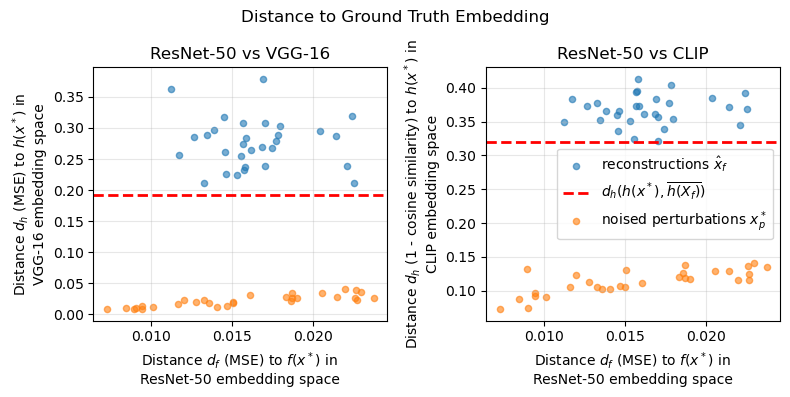
\includegraphics[width=\linewidth]{figures/avg-distance-scatter.png}
    \caption{
       Comparison of embedding distances for noised images, reconstructions and averaged reconstruction embeddings for $f$ being a ResNet backbone, and $h$ being a VGG backbone (left) and $h$ being a CLIP backbone (right).
    }
    \label{fig:avg_distance_scatter}
\end{figure}

That leads to the intuitive assumption the that embeddings under a foreign backbone $h$ scatter around the embedding of the private image $h(x^*)$ and do not deviate in a specific direction.
This idea is illustrated in figure~\ref{fig:avg_embedding_sketch}.
\begin{figure}[ht]
    \centering
    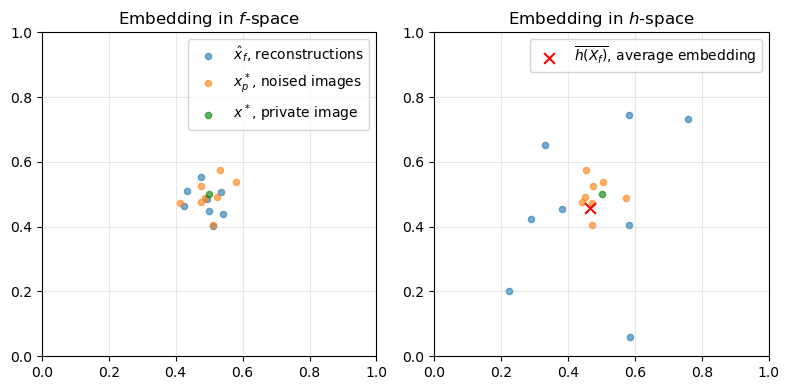
\includegraphics[width=\linewidth]{figures/avg-embedding-sketch.png}
    \caption{
       Illustration of the imagined scattering behavior of embeddings under a backbone used for reconstruction $f$ (left) and a foreign backbone $h$ (right).
       The average embedding in the foreign space is closer to the embedding of the private image than the embeddings of the reconstructions.
    }
    \label{fig:avg_embedding_sketch}
\end{figure}

\subsection{Combining Multiple Backbones}\label{combining_backbones}
To potentially make use of this we explored multiple methods to incorporate the average in the foreign embedding space during the reconstruction process.

Since most of the used networks apply a ReLu activation as their last non-linearity, simply calculating the arithmetic average in each coordinate leads to a huge shift in the shape of the distribution of embeddings.
To reduce that shift, we can perform the averaging in the latent space before applying the last ReLu activation.
The effect of this can bee seen in figure~\ref{fig:relu_norelu_distribution_shift}.
We perform the experiments on both, the truncated and the original backbones.

\begin{figure}[ht]
    \centering
    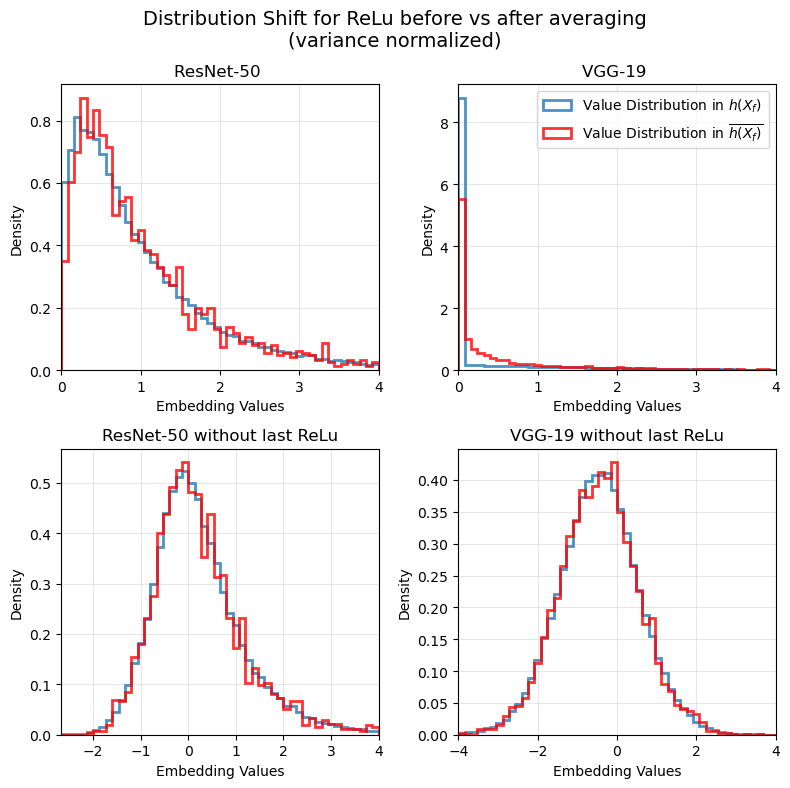
\includegraphics[width=\linewidth]{figures/relu-norelu-distribution-shift.png}
    \caption{
       Distribution of embeddings in different backbones.
       Top: Value distribution under original backbone.
       Bottom: Value distribution under modified backbone with the last ReLu removed.
    }
    \label{fig:relu_norelu_distribution_shift}
\end{figure}

We incorporate the average embedding in a foreign space by extending loss function from equation~\ref{eq:loss_function_base}:
\begin{equation}\label{eq:loss_function}
\mathcal{L}(x, y^*, y_h) = \mathcal{L}_{f}(x, y^*) + \mathcal{L}_{h}(x, y_h) + \mathcal{R}(S_N(x))
\end{equation}
where $\mathcal{L}_{h}$ is defined as in equation~\ref{eq:loss_function_f} and $y_h$ is a element in the foreign space.
We will choose $y_h$ to either be $\overline{h(X^{(t)})}$, the average embedding of the current reconstructions in the foreign space, or $\overline{h(X_f)}$, the average embedding of reconstructions of previously completed reconstruction run with the loss function from equation~\ref{eq:loss_function_base}.

\section{Experiments}
We conducted a series of experiments to evaluate the effectiveness of the proposed method.
We experimented with different choices of the foreign backbone $h$ and the construction of $y_h$.

For the presented experiments we fixed $f$ to be a ResNet-50, pretrained on ImageNet without its classification layer.
For $h$ we explored different ResNet backbones, ResNet-18, ResNet-34, ResNet-50, ResNet-101 and ResNet-152 (referred to as rn18, rn34, rn50, rn101, rn152), VGG-16 and VGG-19 (referred to as vgg16 and vgg19) and a CLIP ViT-L/14 (referred to as clip).
For all of them (except clip) we used a model pretrained on ImageNet without its classification layer and also performed the experiments on the original and the version without the last ReLU activation (denoted by a -nrl suffix).
For the CLIP model, we used an OpenAI pretrained version as presented in~\cite{radfordLearningTransferableVisual2021}.
As metrics for the evaluation of the reconstruction quality we used the structural similarity index measure (SSIM)~\cite{zhouwangImageQualityAssessment2004}, the learned perceptual image patch similarity (LPIPS)~\cite{zhangUnreasonableEffectivenessDeep2018} as well as the cosine similarity based distance to the ground truth CLIP embedding of the image ($\mathcal{L}_{\text{clip}}(\hat x, \text{clip}(x))$).
The SSIM value is supplemented by LPIPS, which is used to measure perceptual similarity, as a human viewer would perceive it and by the CLIP loss, which measures how well the reconstruction captures the semantic content of the original image.


The calculation of $y_h$ was performed by using $m=4$ parallel reconstructions and in the two different ways described in Section~\ref{combining_backbones}:
We choose $y_h$ to be the average of the current iteration ($y_h^\text{avg}=\overline{h(X^{(t)})}$) or to be a reference vector obtained by independently and previously completed run ($y_h^\text{ref}=\overline{h(X_f)}$).
\subsection{Influence of the Last ReLU}
The effect of removing the last ReLU activation can be seen in table~\ref{tab:results_comparison_relu}.
Despite the rather promising observations in figure~\ref{fig:relu_norelu_distribution_shift}, we observe that removing the last ReLU activation generally hurts the reconstruction quality independent of the metric used.

The reason for this could be that removing the last ReLU activation increases the search space of the optimization problem significantly.
This could lead to the optimization getting stuck in local minima more often.
Another reason could be that the last ReLU activation is an important part of the backbone's learned representation and removing it degrades the quality of the features extracted by the backbone.
This is because during training of the backbone the exact value of below zero activations were not relevant and thus not learned but now they contribute directly to the loss.

\subsection{Choice of Foreign Backbone}
The choice of the foreign backbone $h$ has a measurable impact on the reconstruction quality.
We are especially interested in the effect of the depth of the network on the reconstruction quality.
Within the family of ResNets we observe that increasing the depth of the network generally improves the reconstruction quality as can be seen in table~\ref{tab:results_comparison_rn50}.
This may be due to the fact that deeper networks are able to capture more complex features and thus provide a more informative guidance during the reconstruction process.
The same effect can be observed in the family of VGG networks as can be seen in table~\ref{tab:results_comparison_vgg16}.

\subsection{Method of Calculating the Reference Embedding}
Whether using the average of the current reconstructions or a reference vector from a previous run has significant impact on the reconstruction quality as can be seen in table~\ref{tab:results_comparison_avg}.
For the perceptual LPIPS metric and the CLIP based metric we observe a significant improvement when using the ref-method.
This may be due to the fact that in the ref-method the reference vector can be freely developed in a independent run and thus may contain more complex features, while the avg-method pulls the reconstructions towards an average from the beginning of the optimization, which may discourage exploration of more diverse solutions.

On the other hand, the SSIM metric seems to benefit from the avg-method.
This may be due to the same reason: the avg-method discourages complex features and thus reduce the development of strong structural artifacts that may be penalized by the SSIM metric.

For the best performing backbones (rn152, vgg19, clip (each without modification)) and the ref-method we performed additional experiments to evaluate the effect of the number of parallel reconstructions used to calculate $y_h$.
Going from 4 to 8 parallel reconstructions yields an improvement for the VGG and CLIP backbones while the ResNet performance degrades as can be seen in table~\ref{tab:results_comparison_04_to_08_recons}
Doubling the parallel reconstructions again from 8 to 16 continues this trend only partially as can be seen in table~\ref{tab:results_comparison_08_to_16_recons}.

\subsection{Effect of the Data Distribution}
Incorporating foreign backbones $h$ may be especially beneficial if the private image $x^*$ stems from a different distribution than the data used to train the backbone $f$.
To evaluate the effect of incorporating foreign embeddings on the reconstruction quality when reconstructing images from a different distribution than $f$ was trained on, we performed experiments on images from the FFHQ dataset~\cite{karras2019style}.
In table~\ref{tab:results_comparison_in_vs_ffhq} we display how much the reconstruction quality improves for the FFHQ dataset when using different foreign backbones.
In parentheses we display the difference to the corresponding improvement when reconstructing images from the ImageNet validation set.

Especially for reconstructions using a backbone $h$ that has a different architecture than $f$ (e.g. VGG or CLIP) we observe a improvement in reconstruction quality when reconstructing images from the FFHQ dataset compared to the ImageNet validation set.
This may be some form of generalization effect, as the features learned by different architectures may be more general and thus provide a more informative guidance during the reconstruction process, especially for the CLIP model where the training data is more diverse.
\section{Discussion}
\subsection{Results}
Table~\ref{tab:best_rows_comparison} shows the results from the best parametrizations for each architecture.
That means, we chose deepest version for each network and the ReLU was not removed from the backbones, also we used the reference method to calculate $y_h$.
The results do not show a clear improvement over the base method, but there are some improvements in certain metrics for certain backbones.
The fact that using more parallel reconstructions shows only slight improvements or even degrades the performance for some metrics indicates that the aggregation method of simply averaging the embeddings in the foreign space is not optimal.
Also the observed behavior that removing the last ReLU activation generally degrades the performance, despite the observed distribution shift in section~\ref{combining_backbones}, supports this and motivates further research in the direction of better aggregation methods.

Table~\ref{tab:results_comparison_in_vs_ffhq} shows that using foreign backbones seems to be especially beneficial when reconstructing images from a different distribution than the one used to train the backbone $f$, even when $h$ is not trained on the distribution of $x^*$.
Using a backbone trained on a similar distribution as $x^*$ may further increase this effect.

\subsection{Possible Extensions}
This idea can be extended in multiple directions without diverging from the main concept.
Possible extension in direction of how $h$ is chosen include:
\begin{enumerate}
    \item The identity mapping $h(x) = x$ would correspond to averaging the reconstructions in pixel space.
    That could encourage the reconstructions mechanism to maintain common features in pixel space that were already discovered.
    \item Choosing $h$ as an autoencoder trained on a large corpus of images could encourage the reconstructions to maintain features that are common in natural images.
    \item If the attacker has a suspicion about the distribution of the private image, $h$ could be chosen as a backbone trained on a similar distribution.
    \item If the attacker is only interested in the reconstruction of certain parts of the image, $h$ could be chosen as a backbone trained for that specific task (e.g. face recognition).
    \item In the same manner the backbone $f$ could be appended by a task specific head $c$ to encourage the reconstruction of certain features and $h$ can be chosen to be $c \circ f$.
    \item If $x^*$ stems from a different distribution than the data used to train $f$, the effect of using foreign backbones $h$ may increase.
    Especially if $h$ is trained on a distribution similar to the one of $x^*$.
\end{enumerate}
Possible extensions in direction of how $y_h$ is calculated include:
\begin{enumerate}
    \item Instead of using the average embedding in the foreign space, one could use a more robust statistic like the median or a trimmed mean.
    \item One could also use a clustering algorithm to identify groups of similar reconstructions and use the centroid of the largest cluster as $y_h$.
    \item For location sensitive embeddings $h$ (e.g. $h=\text{id}$) using image registration method like RANSAC-Flow~\cite{shenRANSACFlowGenericTwoStage2020} before averaging could be beneficial as this method already was shown to be effective for other reconstruction scenarios as in~\cite{yinSeeGradientsImage2021}.
\end{enumerate}
Extensions towards adjusting the loss and distance functions include:
\begin{enumerate}
    \item Another extension would be to adjust the distance function $d_h$ to punish certain components differently depending on the agreement of the reconstructions in the foreign space in that components.
    \item Combining multiple losses $\mathcal{L}_{h_1}, \mathcal{L}_{h_2}, \dots$ for different backbones $h_1, h_2, \dots$ is a simple but not yet explored extension.
\end{enumerate}


\bibliographystyle{plain}
\bibliography{references}

\begin{table*}[ht]
    \centering
        \begin{tabular}{|l|l|l|c|c|c|c|c|}
\hline
Type & ReLU & $h$ & SSIM $\uparrow$ & LPIPS VGG $\downarrow$ & LPIPS Alex $\downarrow$ & CLIP cos sim $\uparrow$ & \# Runs \\
\hline
\rowcolor{verylightgray}avg & yes & rn18 & \texttt{0.171 {\color{black}(+0.000)}} & \texttt{0.802 {\color{black}(+0.000)}} & \texttt{0.800 {\color{black}(+0.000)}} & \texttt{0.600 {\color{black}(+0.000)}} & \texttt{8} \\
avg & no & rn18 & \texttt{0.171 {\color{black}(+0.000)}} & \texttt{0.811 {\color{red}(+0.009)}} & \texttt{0.822 {\color{red}(+0.022)}} & \texttt{0.590 {\color{red}(-0.011)}} & \texttt{8} \\
\hline
\rowcolor{verylightgray}ref & yes & rn18 & \texttt{0.168 {\color{black}(+0.000)}} & \texttt{0.789 {\color{black}(+0.000)}} & \texttt{0.780 {\color{black}(+0.000)}} & \texttt{0.614 {\color{black}(+0.000)}} & \texttt{8} \\
ref & no & rn18 & \texttt{0.167 {\color{black}(-0.000)}} & \texttt{0.794 {\color{red}(+0.005)}} & \texttt{0.792 {\color{red}(+0.013)}} & \texttt{0.604 {\color{red}(-0.010)}} & \texttt{8} \\
\hline
\rowcolor{verylightgray}avg & yes & rn34 & \texttt{0.171 {\color{black}(+0.000)}} & \texttt{0.796 {\color{black}(+0.000)}} & \texttt{0.794 {\color{black}(+0.000)}} & \texttt{0.577 {\color{black}(+0.000)}} & \texttt{8} \\
avg & no & rn34 & \texttt{0.171 {\color{red}(-0.001)}} & \texttt{0.801 {\color{red}(+0.005)}} & \texttt{0.803 {\color{red}(+0.009)}} & \texttt{0.570 {\color{red}(-0.007)}} & \texttt{8} \\
\hline
\rowcolor{verylightgray}ref & yes & rn34 & \texttt{0.167 {\color{black}(+0.000)}} & \texttt{0.784 {\color{black}(+0.000)}} & \texttt{0.772 {\color{black}(+0.000)}} & \texttt{0.625 {\color{black}(+0.000)}} & \texttt{8} \\
ref & no & rn34 & \texttt{0.165 {\color{red}(-0.002)}} & \texttt{0.789 {\color{red}(+0.005)}} & \texttt{0.780 {\color{red}(+0.008)}} & \texttt{0.616 {\color{red}(-0.010)}} & \texttt{8} \\
\hline
\rowcolor{verylightgray}avg & yes & rn50 & \texttt{0.174 {\color{black}(+0.000)}} & \texttt{0.790 {\color{black}(+0.000)}} & \texttt{0.763 {\color{black}(+0.000)}} & \texttt{0.627 {\color{black}(+0.000)}} & \texttt{8} \\
avg & no & rn50 & \texttt{0.174 {\color{black}(+0.000)}} & \texttt{0.794 {\color{red}(+0.005)}} & \texttt{0.770 {\color{red}(+0.008)}} & \texttt{0.626 {\color{red}(-0.001)}} & \texttt{8} \\
\hline
\rowcolor{verylightgray}ref & yes & rn50 & \texttt{0.173 {\color{black}(+0.000)}} & \texttt{0.781 {\color{black}(+0.000)}} & \texttt{0.754 {\color{black}(+0.000)}} & \texttt{0.636 {\color{black}(+0.000)}} & \texttt{8} \\
ref & no & rn50 & \texttt{0.170 {\color{red}(-0.003)}} & \texttt{0.784 {\color{red}(+0.003)}} & \texttt{0.757 {\color{red}(+0.003)}} & \texttt{0.630 {\color{red}(-0.005)}} & \texttt{8} \\
\hline
\rowcolor{verylightgray}avg & yes & rn101 & \texttt{0.172 {\color{black}(+0.000)}} & \texttt{0.776 {\color{black}(+0.000)}} & \texttt{0.760 {\color{black}(+0.000)}} & \texttt{0.625 {\color{black}(+0.000)}} & \texttt{8} \\
avg & no & rn101 & \texttt{0.172 {\color{black}(-0.000)}} & \texttt{0.780 {\color{red}(+0.004)}} & \texttt{0.768 {\color{red}(+0.008)}} & \texttt{0.619 {\color{red}(-0.006)}} & \texttt{8} \\
\hline
\rowcolor{verylightgray}ref & yes & rn101 & \texttt{0.174 {\color{black}(+0.000)}} & \texttt{0.778 {\color{black}(+0.000)}} & \texttt{0.753 {\color{black}(+0.000)}} & \texttt{0.643 {\color{black}(+0.000)}} & \texttt{8} \\
ref & no & rn101 & \texttt{0.174 {\color{black}(-0.000)}} & \texttt{0.784 {\color{red}(+0.006)}} & \texttt{0.760 {\color{red}(+0.007)}} & \texttt{0.640 {\color{red}(-0.003)}} & \texttt{8} \\
\hline
\rowcolor{verylightgray}avg & yes & rn152 & \texttt{0.173 {\color{black}(+0.000)}} & \texttt{0.780 {\color{black}(+0.000)}} & \texttt{0.761 {\color{black}(+0.000)}} & \texttt{0.624 {\color{black}(+0.000)}} & \texttt{8} \\
avg & no & rn152 & \texttt{0.174 {\color{green}(+0.001)}} & \texttt{0.782 {\color{red}(+0.002)}} & \texttt{0.765 {\color{red}(+0.004)}} & \texttt{0.611 {\color{red}(-0.013)}} & \texttt{8} \\
\hline
\rowcolor{verylightgray}ref & yes & rn152 & \texttt{0.171 {\color{black}(+0.000)}} & \texttt{0.781 {\color{black}(+0.000)}} & \texttt{0.756 {\color{black}(+0.000)}} & \texttt{0.641 {\color{black}(+0.000)}} & \texttt{8} \\
ref & no & rn152 & \texttt{0.171 {\color{green}(+0.001)}} & \texttt{0.782 {\color{red}(+0.001)}} & \texttt{0.755 {\color{green}(-0.001)}} & \texttt{0.641 {\color{red}(-0.001)}} & \texttt{8} \\
\hline
\rowcolor{verylightgray}avg & yes & vgg16 & \texttt{0.174 {\color{black}(+0.000)}} & \texttt{0.789 {\color{black}(+0.000)}} & \texttt{0.780 {\color{black}(+0.000)}} & \texttt{0.615 {\color{black}(+0.000)}} & \texttt{8} \\
avg & no & vgg16 & \texttt{0.180 {\color{green}(+0.005)}} & \texttt{0.850 {\color{red}(+0.061)}} & \texttt{0.870 {\color{red}(+0.090)}} & \texttt{0.560 {\color{red}(-0.055)}} & \texttt{8} \\
\hline
\rowcolor{verylightgray}ref & yes & vgg16 & \texttt{0.179 {\color{black}(+0.000)}} & \texttt{0.787 {\color{black}(+0.000)}} & \texttt{0.770 {\color{black}(+0.000)}} & \texttt{0.625 {\color{black}(+0.000)}} & \texttt{8} \\
ref & no & vgg16 & \texttt{0.176 {\color{red}(-0.003)}} & \texttt{0.816 {\color{red}(+0.029)}} & \texttt{0.802 {\color{red}(+0.032)}} & \texttt{0.569 {\color{red}(-0.056)}} & \texttt{8} \\
\hline
\rowcolor{verylightgray}avg & yes & vgg19 & \texttt{0.174 {\color{black}(+0.000)}} & \texttt{0.779 {\color{black}(+0.000)}} & \texttt{0.763 {\color{black}(+0.000)}} & \texttt{0.616 {\color{black}(+0.000)}} & \texttt{8} \\
avg & no & vgg19 & \texttt{0.171 {\color{red}(-0.004)}} & \texttt{0.864 {\color{red}(+0.085)}} & \texttt{0.848 {\color{red}(+0.085)}} & \texttt{0.555 {\color{red}(-0.061)}} & \texttt{8} \\
\hline
\rowcolor{verylightgray}ref & yes & vgg19 & \texttt{0.177 {\color{black}(+0.000)}} & \texttt{0.782 {\color{black}(+0.000)}} & \texttt{0.770 {\color{black}(+0.000)}} & \texttt{0.633 {\color{black}(+0.000)}} & \texttt{8} \\
ref & no & vgg19 & \texttt{0.176 {\color{red}(-0.001)}} & \texttt{0.812 {\color{red}(+0.030)}} & \texttt{0.810 {\color{red}(+0.040)}} & \texttt{0.600 {\color{red}(-0.033)}} & \texttt{8} \\
\hline
\rowcolor{verylightgray}avg & yes & clip & \texttt{0.167 {\color{black}(+0.000)}} & \texttt{0.797 {\color{black}(+0.000)}} & \texttt{0.764 {\color{black}(+0.000)}} & \texttt{0.568 {\color{black}(+0.000)}} & \texttt{8} \\
avg & no & clip & \texttt{0.168 {\color{black}(+0.000)}} & \texttt{0.797 {\color{black}(-0.000)}} & \texttt{0.764 {\color{black}(+0.000)}} & \texttt{0.572 {\color{green}(+0.003)}} & \texttt{8} \\
\hline
\rowcolor{verylightgray}ref & yes & clip & \texttt{0.162 {\color{black}(+0.000)}} & \texttt{0.786 {\color{black}(+0.000)}} & \texttt{0.766 {\color{black}(+0.000)}} & \texttt{0.654 {\color{black}(+0.000)}} & \texttt{8} \\
ref & no & clip & \texttt{0.162 {\color{red}(-0.001)}} & \texttt{0.786 {\color{black}(+0.000)}} & \texttt{0.768 {\color{red}(+0.002)}} & \texttt{0.662 {\color{green}(+0.008)}} & \texttt{8} \\
\hline
\end{tabular}

        \caption{
            Comparison of reconstruction quality with and without the last ReLU activation.
            The differences are calculated with respect to the same backbone and $y_h$ configuration so that only the effect of the removal of the ReLU is shown.
            Reference lines are indicated by a gray background.
        }
        \label{tab:results_comparison_relu}
\end{table*}

\begin{table*}[ht]
    \centering
        \begin{tabular}{|l|l|l|c|c|c|c|c|}
\hline
Type & ReLU & $h$ & SSIM $\uparrow$ & LPIPS VGG $\downarrow$ & LPIPS Alex $\downarrow$ & CLIP cos sim $\uparrow$ & \# Runs \\
\hline
avg & yes & rn18 & \texttt{0.171 {\color{red}(-0.003)}} & \texttt{0.802 {\color{red}(+0.012)}} & \texttt{0.800 {\color{red}(+0.037)}} & \texttt{0.600 {\color{red}(-0.027)}} & \texttt{8} \\
avg & no & rn18 & \texttt{0.171 {\color{red}(-0.003)}} & \texttt{0.811 {\color{red}(+0.016)}} & \texttt{0.822 {\color{red}(+0.051)}} & \texttt{0.590 {\color{red}(-0.037)}} & \texttt{8} \\
ref & yes & rn18 & \texttt{0.168 {\color{red}(-0.005)}} & \texttt{0.789 {\color{red}(+0.008)}} & \texttt{0.780 {\color{red}(+0.026)}} & \texttt{0.614 {\color{red}(-0.022)}} & \texttt{8} \\
ref & no & rn18 & \texttt{0.167 {\color{red}(-0.002)}} & \texttt{0.794 {\color{red}(+0.010)}} & \texttt{0.792 {\color{red}(+0.035)}} & \texttt{0.604 {\color{red}(-0.027)}} & \texttt{8} \\
\hline
avg & yes & rn34 & \texttt{0.171 {\color{red}(-0.003)}} & \texttt{0.796 {\color{red}(+0.006)}} & \texttt{0.794 {\color{red}(+0.032)}} & \texttt{0.577 {\color{red}(-0.050)}} & \texttt{8} \\
avg & no & rn34 & \texttt{0.171 {\color{red}(-0.003)}} & \texttt{0.801 {\color{red}(+0.007)}} & \texttt{0.803 {\color{red}(+0.033)}} & \texttt{0.570 {\color{red}(-0.056)}} & \texttt{8} \\
ref & yes & rn34 & \texttt{0.167 {\color{red}(-0.006)}} & \texttt{0.784 {\color{red}(+0.003)}} & \texttt{0.772 {\color{red}(+0.018)}} & \texttt{0.625 {\color{red}(-0.010)}} & \texttt{8} \\
ref & no & rn34 & \texttt{0.165 {\color{red}(-0.004)}} & \texttt{0.789 {\color{red}(+0.005)}} & \texttt{0.780 {\color{red}(+0.023)}} & \texttt{0.616 {\color{red}(-0.015)}} & \texttt{8} \\
\hline
\rowcolor{verylightgray}avg & yes & rn50 & \texttt{0.174 {\color{black}(+0.000)}} & \texttt{0.790 {\color{black}(+0.000)}} & \texttt{0.763 {\color{black}(+0.000)}} & \texttt{0.627 {\color{black}(+0.000)}} & \texttt{8} \\
\rowcolor{verylightgray}avg & no & rn50 & \texttt{0.174 {\color{black}(+0.000)}} & \texttt{0.794 {\color{black}(+0.000)}} & \texttt{0.770 {\color{black}(+0.000)}} & \texttt{0.626 {\color{black}(+0.000)}} & \texttt{8} \\
\rowcolor{verylightgray}ref & yes & rn50 & \texttt{0.173 {\color{black}(+0.000)}} & \texttt{0.781 {\color{black}(+0.000)}} & \texttt{0.754 {\color{black}(+0.000)}} & \texttt{0.636 {\color{black}(+0.000)}} & \texttt{8} \\
\rowcolor{verylightgray}ref & no & rn50 & \texttt{0.170 {\color{black}(+0.000)}} & \texttt{0.784 {\color{black}(+0.000)}} & \texttt{0.757 {\color{black}(+0.000)}} & \texttt{0.630 {\color{black}(+0.000)}} & \texttt{8} \\
\hline
avg & yes & rn101 & \texttt{0.172 {\color{red}(-0.002)}} & \texttt{0.776 {\color{green}(-0.014)}} & \texttt{0.760 {\color{green}(-0.002)}} & \texttt{0.625 {\color{red}(-0.002)}} & \texttt{8} \\
avg & no & rn101 & \texttt{0.172 {\color{red}(-0.003)}} & \texttt{0.780 {\color{green}(-0.014)}} & \texttt{0.768 {\color{green}(-0.003)}} & \texttt{0.619 {\color{red}(-0.008)}} & \texttt{8} \\
ref & yes & rn101 & \texttt{0.174 {\color{green}(+0.002)}} & \texttt{0.778 {\color{green}(-0.003)}} & \texttt{0.753 {\color{green}(-0.001)}} & \texttt{0.643 {\color{green}(+0.007)}} & \texttt{8} \\
ref & no & rn101 & \texttt{0.174 {\color{green}(+0.005)}} & \texttt{0.784 {\color{black}(+0.000)}} & \texttt{0.760 {\color{red}(+0.003)}} & \texttt{0.640 {\color{green}(+0.010)}} & \texttt{8} \\
\hline
avg & yes & rn152 & \texttt{0.173 {\color{red}(-0.001)}} & \texttt{0.780 {\color{green}(-0.010)}} & \texttt{0.761 {\color{green}(-0.002)}} & \texttt{0.624 {\color{red}(-0.003)}} & \texttt{8} \\
avg & no & rn152 & \texttt{0.174 {\color{red}(-0.001)}} & \texttt{0.782 {\color{green}(-0.013)}} & \texttt{0.765 {\color{green}(-0.006)}} & \texttt{0.611 {\color{red}(-0.015)}} & \texttt{8} \\
ref & yes & rn152 & \texttt{0.171 {\color{red}(-0.002)}} & \texttt{0.781 {\color{black}(-0.000)}} & \texttt{0.756 {\color{red}(+0.002)}} & \texttt{0.641 {\color{green}(+0.006)}} & \texttt{8} \\
ref & no & rn152 & \texttt{0.171 {\color{green}(+0.002)}} & \texttt{0.782 {\color{green}(-0.002)}} & \texttt{0.755 {\color{green}(-0.002)}} & \texttt{0.641 {\color{green}(+0.010)}} & \texttt{8} \\
\hline
\end{tabular}

        \caption{
            Comparison of different depths of ResNets.
            ResNet-50 is chosen as the reference value for the differences.
            Reference lines are indicated by a gray background.
        }
        \label{tab:results_comparison_rn50}
\end{table*}

\begin{table*}[ht]
    \centering
        \begin{tabular}{|l|l|l|c|c|c|c|c|}
\hline
Type & ReLU & $h$ & SSIM $\uparrow$ & LPIPS VGG $\downarrow$ & LPIPS Alex $\downarrow$ & CLIP cos sim $\uparrow$ & \# Runs \\
\hline
\rowcolor{verylightgray}avg & yes & vgg16 & \texttt{0.174 {\color{black}(+0.000)}} & \texttt{0.789 {\color{black}(+0.000)}} & \texttt{0.780 {\color{black}(+0.000)}} & \texttt{0.615 {\color{black}(+0.000)}} & \texttt{8} \\
\rowcolor{verylightgray}avg & no & vgg16 & \texttt{0.180 {\color{black}(+0.000)}} & \texttt{0.850 {\color{black}(+0.000)}} & \texttt{0.870 {\color{black}(+0.000)}} & \texttt{0.560 {\color{black}(+0.000)}} & \texttt{8} \\
\rowcolor{verylightgray}ref & yes & vgg16 & \texttt{0.179 {\color{black}(+0.000)}} & \texttt{0.787 {\color{black}(+0.000)}} & \texttt{0.770 {\color{black}(+0.000)}} & \texttt{0.625 {\color{black}(+0.000)}} & \texttt{8} \\
\rowcolor{verylightgray}ref & no & vgg16 & \texttt{0.176 {\color{black}(+0.000)}} & \texttt{0.816 {\color{black}(+0.000)}} & \texttt{0.802 {\color{black}(+0.000)}} & \texttt{0.569 {\color{black}(+0.000)}} & \texttt{8} \\
\hline
avg & yes & vgg19 & \texttt{0.174 {\color{black}(-0.000)}} & \texttt{0.779 {\color{green}(-0.010)}} & \texttt{0.763 {\color{green}(-0.017)}} & \texttt{0.616 {\color{black}(+0.000)}} & \texttt{8} \\
avg & no & vgg19 & \texttt{0.171 {\color{red}(-0.009)}} & \texttt{0.864 {\color{red}(+0.014)}} & \texttt{0.848 {\color{green}(-0.022)}} & \texttt{0.555 {\color{red}(-0.005)}} & \texttt{8} \\
ref & yes & vgg19 & \texttt{0.177 {\color{red}(-0.002)}} & \texttt{0.782 {\color{green}(-0.005)}} & \texttt{0.770 {\color{black}(+0.000)}} & \texttt{0.633 {\color{green}(+0.008)}} & \texttt{8} \\
ref & no & vgg19 & \texttt{0.176 {\color{black}(+0.000)}} & \texttt{0.812 {\color{green}(-0.004)}} & \texttt{0.810 {\color{red}(+0.008)}} & \texttt{0.600 {\color{green}(+0.031)}} & \texttt{8} \\
\hline
\end{tabular}

        \caption{
            Comparison of different depths of VGGs.
            VGG-16 is chosen as the reference value for the differences.
            Reference lines are indicated by a gray background.
        }
        \label{tab:results_comparison_vgg16}
\end{table*}

\begin{table*}[ht]
    \centering
        \begin{tabular}{|l|l|l|c|c|c|c|c|}
\hline
Type & ReLU & $h$ & SSIM $\uparrow$ & LPIPS VGG $\downarrow$ & LPIPS Alex $\downarrow$ & CLIP cos sim $\uparrow$ & $m$ \\
\hline
\rowcolor{verylightgray}avg & yes & rn18 & \texttt{0.176 {\color{black}(+0.000)}} & \texttt{0.793 {\color{black}(+0.000)}} & \texttt{0.796 {\color{black}(+0.000)}} & \texttt{0.600 {\color{black}(+0.000)}} & \texttt{4} \\
\rowcolor{verylightgray}avg & no & rn18 & \texttt{0.176 {\color{black}(+0.000)}} & \texttt{0.817 {\color{black}(+0.000)}} & \texttt{0.807 {\color{black}(+0.000)}} & \texttt{0.595 {\color{black}(+0.000)}} & \texttt{4} \\
\hline
ref & yes & rn18 & \texttt{0.170 {\color{red}(-0.006)}} & \texttt{0.778 {\color{green}(-0.015)}} & \texttt{0.786 {\color{green}(-0.009)}} & \texttt{0.621 {\color{green}(+0.021)}} & \texttt{4} \\
ref & no & rn18 & \texttt{0.168 {\color{red}(-0.008)}} & \texttt{0.795 {\color{green}(-0.022)}} & \texttt{0.793 {\color{green}(-0.014)}} & \texttt{0.603 {\color{green}(+0.007)}} & \texttt{4} \\
\hline
\rowcolor{verylightgray}avg & yes & rn34 & \texttt{0.175 {\color{black}(+0.000)}} & \texttt{0.792 {\color{black}(+0.000)}} & \texttt{0.794 {\color{black}(+0.000)}} & \texttt{0.585 {\color{black}(+0.000)}} & \texttt{4} \\
\rowcolor{verylightgray}avg & no & rn34 & \texttt{0.173 {\color{black}(+0.000)}} & \texttt{0.800 {\color{black}(+0.000)}} & \texttt{0.795 {\color{black}(+0.000)}} & \texttt{0.576 {\color{black}(+0.000)}} & \texttt{4} \\
\hline
ref & yes & rn34 & \texttt{0.166 {\color{red}(-0.009)}} & \texttt{0.776 {\color{green}(-0.016)}} & \texttt{0.791 {\color{green}(-0.003)}} & \texttt{0.623 {\color{green}(+0.038)}} & \texttt{4} \\
ref & no & rn34 & \texttt{0.166 {\color{red}(-0.007)}} & \texttt{0.783 {\color{green}(-0.017)}} & \texttt{0.793 {\color{green}(-0.001)}} & \texttt{0.606 {\color{green}(+0.030)}} & \texttt{4} \\
\hline
\rowcolor{verylightgray}avg & yes & rn50 & \texttt{0.178 {\color{black}(+0.000)}} & \texttt{0.761 {\color{black}(+0.000)}} & \texttt{0.787 {\color{black}(+0.000)}} & \texttt{0.636 {\color{black}(+0.000)}} & \texttt{4} \\
\rowcolor{verylightgray}avg & no & rn50 & \texttt{0.178 {\color{black}(+0.000)}} & \texttt{0.767 {\color{black}(+0.000)}} & \texttt{0.789 {\color{black}(+0.000)}} & \texttt{0.628 {\color{black}(+0.000)}} & \texttt{4} \\
\hline
ref & yes & rn50 & \texttt{0.175 {\color{red}(-0.003)}} & \texttt{0.755 {\color{green}(-0.006)}} & \texttt{0.779 {\color{green}(-0.008)}} & \texttt{0.636 {\color{black}(-0.000)}} & \texttt{4} \\
ref & no & rn50 & \texttt{0.175 {\color{red}(-0.003)}} & \texttt{0.757 {\color{green}(-0.010)}} & \texttt{0.782 {\color{green}(-0.007)}} & \texttt{0.640 {\color{green}(+0.011)}} & \texttt{4} \\
\hline
\rowcolor{verylightgray}avg & yes & rn101 & \texttt{0.178 {\color{black}(+0.000)}} & \texttt{0.761 {\color{black}(+0.000)}} & \texttt{0.778 {\color{black}(+0.000)}} & \texttt{0.631 {\color{black}(+0.000)}} & \texttt{4} \\
\rowcolor{verylightgray}avg & no & rn101 & \texttt{0.178 {\color{black}(+0.000)}} & \texttt{0.767 {\color{black}(+0.000)}} & \texttt{0.780 {\color{black}(+0.000)}} & \texttt{0.618 {\color{black}(+0.000)}} & \texttt{4} \\
\hline
ref & yes & rn101 & \texttt{0.177 {\color{red}(-0.001)}} & \texttt{0.757 {\color{green}(-0.003)}} & \texttt{0.776 {\color{green}(-0.002)}} & \texttt{0.648 {\color{green}(+0.017)}} & \texttt{4} \\
ref & no & rn101 & \texttt{0.174 {\color{red}(-0.004)}} & \texttt{0.759 {\color{green}(-0.008)}} & \texttt{0.781 {\color{red}(+0.001)}} & \texttt{0.636 {\color{green}(+0.017)}} & \texttt{4} \\
\hline
\rowcolor{verylightgray}avg & yes & rn152 & \texttt{0.178 {\color{black}(+0.000)}} & \texttt{0.760 {\color{black}(+0.000)}} & \texttt{0.777 {\color{black}(+0.000)}} & \texttt{0.627 {\color{black}(+0.000)}} & \texttt{4} \\
\rowcolor{verylightgray}avg & no & rn152 & \texttt{0.176 {\color{black}(+0.000)}} & \texttt{0.766 {\color{black}(+0.000)}} & \texttt{0.781 {\color{black}(+0.000)}} & \texttt{0.619 {\color{black}(+0.000)}} & \texttt{4} \\
\hline
ref & yes & rn152 & \texttt{0.173 {\color{red}(-0.004)}} & \texttt{0.755 {\color{green}(-0.005)}} & \texttt{0.775 {\color{green}(-0.003)}} & \texttt{0.645 {\color{green}(+0.018)}} & \texttt{4} \\
ref & no & rn152 & \texttt{0.177 {\color{black}(+0.000)}} & \texttt{0.756 {\color{green}(-0.010)}} & \texttt{0.776 {\color{green}(-0.005)}} & \texttt{0.643 {\color{green}(+0.024)}} & \texttt{4} \\
\hline
\rowcolor{verylightgray}avg & yes & vgg16 & \texttt{0.176 {\color{black}(+0.000)}} & \texttt{0.779 {\color{black}(+0.000)}} & \texttt{0.787 {\color{black}(+0.000)}} & \texttt{0.616 {\color{black}(+0.000)}} & \texttt{4} \\
\rowcolor{verylightgray}avg & no & vgg16 & \texttt{0.184 {\color{black}(+0.000)}} & \texttt{0.864 {\color{black}(+0.000)}} & \texttt{0.847 {\color{black}(+0.000)}} & \texttt{0.565 {\color{black}(+0.000)}} & \texttt{4} \\
\hline
ref & yes & vgg16 & \texttt{0.182 {\color{green}(+0.005)}} & \texttt{0.775 {\color{green}(-0.004)}} & \texttt{0.788 {\color{red}(+0.001)}} & \texttt{0.621 {\color{green}(+0.005)}} & \texttt{4} \\
ref & no & vgg16 & \texttt{0.173 {\color{red}(-0.011)}} & \texttt{0.803 {\color{green}(-0.061)}} & \texttt{0.813 {\color{green}(-0.034)}} & \texttt{0.570 {\color{green}(+0.005)}} & \texttt{4} \\
\hline
\rowcolor{verylightgray}avg & yes & vgg19 & \texttt{0.178 {\color{black}(+0.000)}} & \texttt{0.767 {\color{black}(+0.000)}} & \texttt{0.785 {\color{black}(+0.000)}} & \texttt{0.616 {\color{black}(+0.000)}} & \texttt{4} \\
\rowcolor{verylightgray}avg & no & vgg19 & \texttt{0.175 {\color{black}(+0.000)}} & \texttt{0.841 {\color{black}(+0.000)}} & \texttt{0.854 {\color{black}(+0.000)}} & \texttt{0.563 {\color{black}(+0.000)}} & \texttt{4} \\
\hline
ref & yes & vgg19 & \texttt{0.181 {\color{green}(+0.003)}} & \texttt{0.775 {\color{red}(+0.007)}} & \texttt{0.785 {\color{black}(-0.000)}} & \texttt{0.634 {\color{green}(+0.019)}} & \texttt{4} \\
ref & no & vgg19 & \texttt{0.175 {\color{black}(-0.000)}} & \texttt{0.812 {\color{green}(-0.029)}} & \texttt{0.810 {\color{green}(-0.044)}} & \texttt{0.593 {\color{green}(+0.029)}} & \texttt{4} \\
\hline
\rowcolor{verylightgray}avg & yes & clip & \texttt{0.173 {\color{black}(+0.000)}} & \texttt{0.761 {\color{black}(+0.000)}} & \texttt{0.793 {\color{black}(+0.000)}} & \texttt{0.573 {\color{black}(+0.000)}} & \texttt{4} \\
\rowcolor{verylightgray}avg & no & clip & \texttt{0.170 {\color{black}(+0.000)}} & \texttt{0.764 {\color{black}(+0.000)}} & \texttt{0.796 {\color{black}(+0.000)}} & \texttt{0.581 {\color{black}(+0.000)}} & \texttt{4} \\
\hline
ref & yes & clip & \texttt{0.167 {\color{red}(-0.006)}} & \texttt{0.769 {\color{red}(+0.007)}} & \texttt{0.788 {\color{green}(-0.005)}} & \texttt{0.661 {\color{green}(+0.088)}} & \texttt{4} \\
ref & no & clip & \texttt{0.163 {\color{red}(-0.007)}} & \texttt{0.768 {\color{red}(+0.004)}} & \texttt{0.788 {\color{green}(-0.008)}} & \texttt{0.648 {\color{green}(+0.067)}} & \texttt{4} \\
\hline
\end{tabular}

        \caption{
            Comparison of different methods of calculating $y_h$ (avg vs ref).
            The differences are calculated with respect to the same backbone and relu configuration so that only the effect of the method of calculating $y_h$ is shown.
            Reference lines are indicated by a gray background.
        }
        \label{tab:results_comparison_avg}
\end{table*}

\begin{table*}[ht]
    \centering
        \begin{tabular}{|l|l|l|c|c|c|c|c|}
\hline
Type & ReLU & $h$ & SSIM $\uparrow$ & LPIPS VGG $\downarrow$ & LPIPS Alex $\downarrow$ & CLIP cos sim $\uparrow$ & $m$ \\
\hline
ref & no & rn152 & \texttt{0.172 {\color{red}(-0.005)}} & \texttt{0.755 {\color{green}(-0.001)}} & \texttt{0.780 {\color{red}(+0.004)}} & \texttt{0.641 {\color{red}(-0.003)}} & \texttt{8} \\
\hline
ref & no & vgg19 & \texttt{0.175 {\color{black}(+0.000)}} & \texttt{0.811 {\color{green}(-0.001)}} & \texttt{0.811 {\color{black}(+0.000)}} & \texttt{0.596 {\color{green}(+0.004)}} & \texttt{8} \\
\hline
ref & no & clip & \texttt{0.164 {\color{green}(+0.001)}} & \texttt{0.766 {\color{green}(-0.002)}} & \texttt{0.782 {\color{green}(-0.005)}} & \texttt{0.655 {\color{green}(+0.007)}} & \texttt{8} \\
\hline
\end{tabular}

        \caption{
        Metrics for 8 parallel reconstructions to calculate $y_h$.
        The differences are calculated with respect to using 4 parallel reconstructions.
        }
        \label{tab:results_comparison_04_to_08_recons}
\end{table*}

\begin{table*}[ht]
    \centering
        \begin{tabular}{|l|l|l|c|c|c|c|c|}
\hline
Type & ReLU & $h$ & SSIM $\uparrow$ & LPIPS VGG $\downarrow$ & LPIPS Alex $\downarrow$ & CLIP cos sim $\uparrow$ & \# Runs \\
\hline
ref & no & rn152 & \texttt{0.172 {\color{black}(+0.000)}} & \texttt{0.782 {\color{red}(+0.001)}} & \texttt{0.755 {\color{black}(-0.000)}} & \texttt{0.641 {\color{black}(+0.000)}} & \texttt{8} \\
\hline
ref & no & vgg19 & \texttt{0.176 {\color{green}(+0.001)}} & \texttt{0.812 {\color{red}(+0.002)}} & \texttt{0.810 {\color{green}(-0.001)}} & \texttt{0.599 {\color{green}(+0.003)}} & \texttt{8} \\
\hline
ref & no & clip & \texttt{0.161 {\color{red}(-0.003)}} & \texttt{0.787 {\color{red}(+0.004)}} & \texttt{0.768 {\color{red}(+0.002)}} & \texttt{0.662 {\color{green}(+0.007)}} & \texttt{8} \\
\hline
\end{tabular}

        \caption{
        Metrics for 16 parallel reconstructions to calculate $y_h$.
        The differences are calculated with respect to using 8 parallel reconstructions.
        }
        \label{tab:results_comparison_08_to_16_recons}
\end{table*}

\begin{table*}[ht]
    \centering
        \begin{tabular}{|l|l|l|c|c|c|c|c|}
\hline
Type & ReLU & $h$ & SSIM $\uparrow$ & LPIPS VGG $\downarrow$ & LPIPS Alex $\downarrow$ & CLIP cos sim $\uparrow$ & $m$ \\
\hline
ref & no & rn152 & \texttt{-0.003 {\color{red}(-0.003)}} & \texttt{-0.004 {\color{green}(-0.009)}} & \texttt{-0.007 {\color{green}(-0.005)}} & \texttt{0.001 {\color{red}(-0.002)}} & \texttt{4} \\
\hline
ref & no & vgg19 & \texttt{0.007 {\color{green}(+0.010)}} & \texttt{0.061 {\color{black}(-0.000)}} & \texttt{0.029 {\color{green}(-0.004)}} & \texttt{-0.018 {\color{green}(+0.030)}} & \texttt{4} \\
\hline
ref & no & clip & \texttt{-0.014 {\color{black}(+0.000)}} & \texttt{0.009 {\color{green}(-0.009)}} & \texttt{0.001 {\color{green}(-0.009)}} & \texttt{0.008 {\color{green}(+0.001)}} & \texttt{4} \\
\hline
\end{tabular}

        \caption{
        Comparison of reconstruction quality improvement when reconstructing images from the FFHQ dataset instead of the ImageNet validation set.
        The values indicate the difference in the corresponding metric compared to the baseline method on FFHQ data.
        The numbers in parentheses indicate the difference to the corresponding improvement when reconstructing images from the ImageNet validation set.
        }
        \label{tab:results_comparison_in_vs_ffhq}
\end{table*}

\begin{table*}[ht]
    \centering
        \begin{tabular}{|l|l|l|c|c|c|c|c|}
\hline
Type & ReLU & $h$ & SSIM $\uparrow$ & LPIPS VGG $\downarrow$ & LPIPS Alex $\downarrow$ & CLIP cos sim $\uparrow$ & $m$ \\
\hline
\rowcolor{verylightgray}baseline & yes & -- & \texttt{0.177 {\color{black}(+0.000)}} & \texttt{0.751 {\color{black}(+0.000)}} & \texttt{0.778 {\color{black}(+0.000)}} & \texttt{0.641 {\color{black}(+0.000)}} & \texttt{4} \\
\hline
ref & yes & rn152 & \texttt{0.173 {\color{red}(-0.003)}} & \texttt{0.755 {\color{red}(+0.004)}} & \texttt{0.775 {\color{green}(-0.004)}} & \texttt{0.645 {\color{green}(+0.005)}} & \texttt{4} \\
\hline
ref & yes & vgg19 & \texttt{0.181 {\color{green}(+0.004)}} & \texttt{0.775 {\color{red}(+0.024)}} & \texttt{0.785 {\color{red}(+0.006)}} & \texttt{0.634 {\color{red}(-0.006)}} & \texttt{4} \\
\hline
ref & no & clip & \texttt{0.163 {\color{red}(-0.014)}} & \texttt{0.768 {\color{red}(+0.017)}} & \texttt{0.788 {\color{red}(+0.010)}} & \texttt{0.648 {\color{green}(+0.007)}} & \texttt{4} \\
\hline
\end{tabular}

        \caption{
            Comparison of reconstruction quality for different the best parametrizations for each architecture.
            Each reported value is the average over 8 different images chosen randomly from the imagenet validation set.
            For each of the images 4 reconstructions were performed and their metrics were averaged.
        }
        \label{tab:best_rows_comparison}
\end{table*}
\end{document}